\chapter{Attention Mechanism}
\section{Introduction}
In this section, we will focus on the deep learning models, the first one being a bidirectional LSTM and the second one an attention layer is added to this LSTM. But it is need to use an other text embedding in order to work with LSTM. Indeed, tf-idf create a sparse matrix with each row corresponding to a value for a given word. This means that the order of the words are lost. In order to solve this, word2vec\cite{Mikolov2013} is used. It allows to match words to continuous vectors of a given size with interesting properties. An other methods, which consist in making word embedding as tuning parameters will be used.

\section{Text to Vectors}
\subsection{Word2Vec}
Word2Vec comes in two fashions: continuous bag of word (CBOW) and skip-gram. It is originaly designed to predic a word given a context. For instance, given two previous words and the two next words, which word is the most likely to take place between them. But it appears that the hidden representation of these words works well as word embedding and have very interesing properties such that words with similar meaning have similar vector representation. It is also possible to perform arithmetic that captures informations such as singular, plural or even capital and countries. For example, we have that $dog - dogs \approx cat - cats$ but also $Paris - France \approx Berlin - Germany$. \\

It is possible to visualize these relasionships by using t-SNE for projecting high dimentions word vectors in 2D space. The results of various relashionships can be see at \textbf{Figure \ref{fig:chap4:word2vec}}.
\begin{figure*}
	\centering
	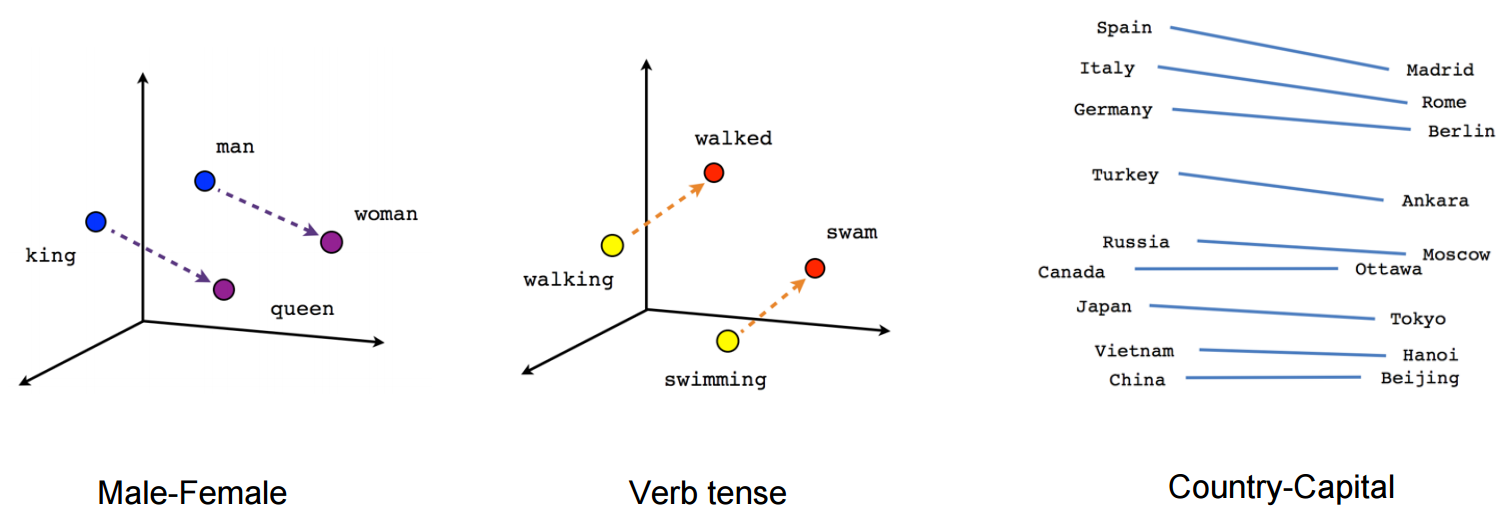
\includegraphics[width=\textwidth]{images/chapitre4/linear-relationships}
	\caption{Relashionships between different words with t-SNE dimentionality reduciton. }
	\label{fig:chap4:word2vec}
\end{figure*}

\subsubsection{How does it works?} 
As the orignal authors did not inteded this kind of results, Xin Rong\cite{Rong2014} did a good job explaing how it works. 

Let V be the size of the vocabulary and that there is only one word in the CBOW model, it give \textbf{Figure \ref{fig:chap4:CBOW}} model. 

\begin{figure*}
	\centering
	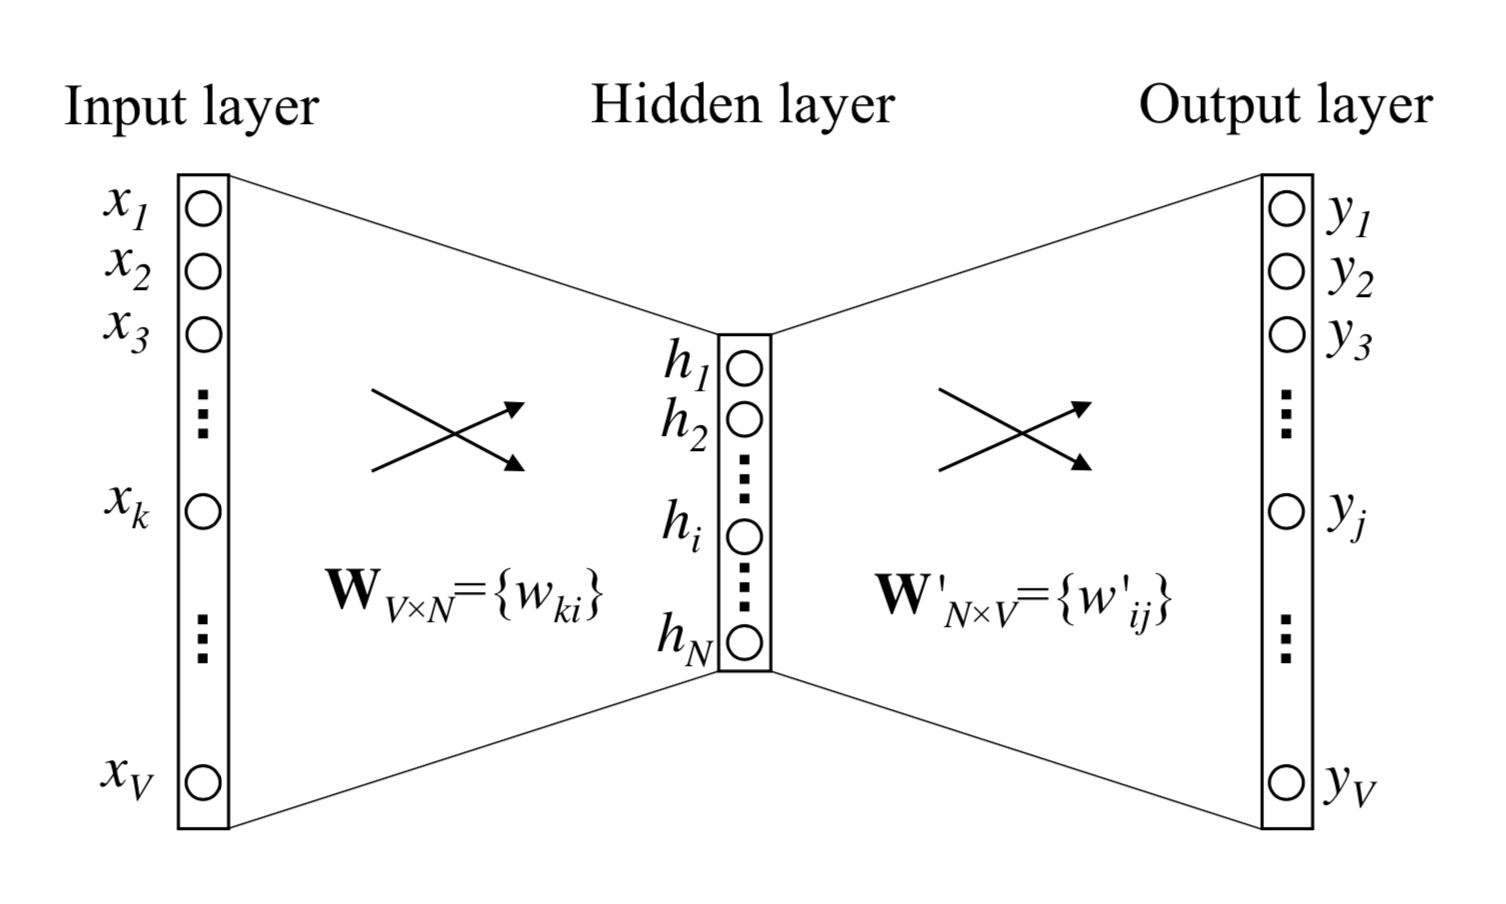
\includegraphics[width=\textwidth]{images/chapitre4/CBOW}
	\caption{A simple CBOW model with only one word in the context}
	\label{fig:chap4:CBOW}
\end{figure*}

Each words is encoded as a one-hot vector of size V. That means that it is a sparse vector full of zeros except for the position assigned to that word which is one. The hidden layers is computed as 
\begin{equation}
	\mathbf{h} = \mathbf{W^Tx}
\end{equation}

Where $\mathbf{W^{V \times N}}$ is the weighte matrix to optimize over. 

The output layer values are computed as 
\begin{equation}
	\mathbf{Y} = \mathbf{W'^Th}
\end{equation}

As before $\mathbf{W'^{N \times V}}$ is also a weight matrix to optimize. The loss can be computed as softmax cross entropy. \\

It is also possible to make the oposite: predicting the context given a single input word. This is the skip-gram model. In this case the loss become \textbf{Equation \ref{eq:loss}}.

\begin{equation}
	E = - \sum_{c=1}^C u_{j^*_c} + C \cdot \sum_{j' = 1}^V \exp(u_{j'}) \ \label{eq:loss}
\end{equation}

$j_c^*$ is the index of the cth output context word and $u_{j^*_c}$ is the score of the jth word in the vocabulary for the cth context word. Finly, the embedding that is used are the value of the hidden layers produced for a given word. 

\begin{figure*}
	\centering
	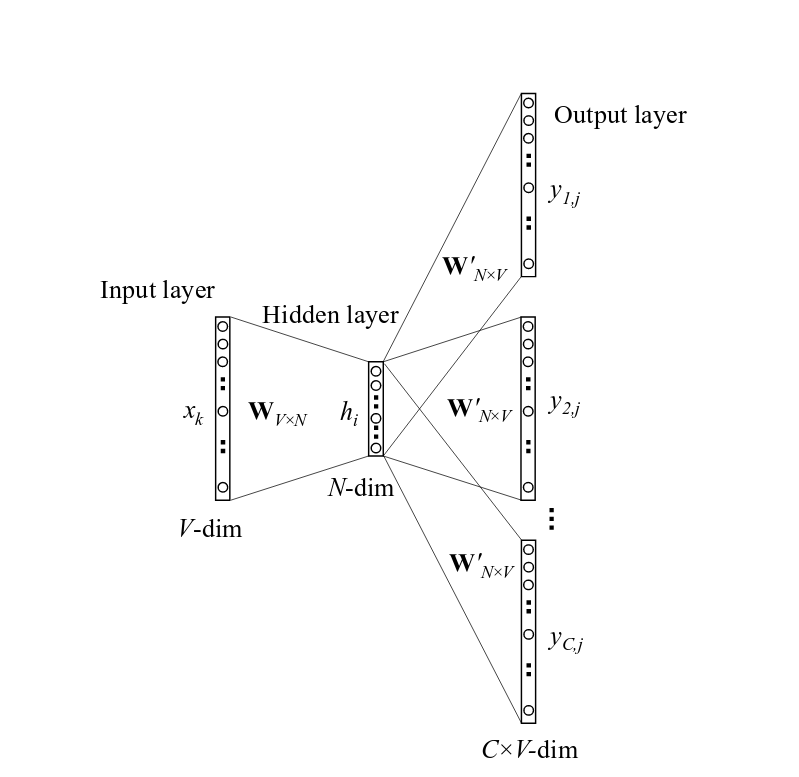
\includegraphics[width=\textwidth]{images/chapitre4/skip-gram}
	\caption{Skip-gram model with multiple outputs.}
	\label{fig:chap4:skip-gram}
\end{figure*}
\section{LSTM}
LSTM or Long Short Term Memory\cite{Hochreiter1997LongSM} is a kind of reccurent neural network that fits well to temporal or sequential input such as texts. A RNN is a type of neural network where the hidden state is fed in a loop with the sequential inputs. There are usualy shown as unrolled version of it (\textbf{Figure \ref{fig:chap4:RNN_unroll}}). Each of the $X_i$ being one value in the sequence.\\

In this case, $X_i$ values are word vectors. There are two possibilities, either use pre-trained vector with word2vec or make $X_i$ inputs a paramter to learn in the same way as it works for the Word2Vec algorithm, having a one-hot enconding of the word and a matrix of weights to tune. Each methods will be used. \\

Recurrent Neural Networks does not works very well with long-term dependencies, that is why LSTM have been introduced. It is made of an input gate, an output gate and a forget gate that are combined in \textbf{Equation \ref{eq:LSTM}}.

\begin{figure}
	\centering
	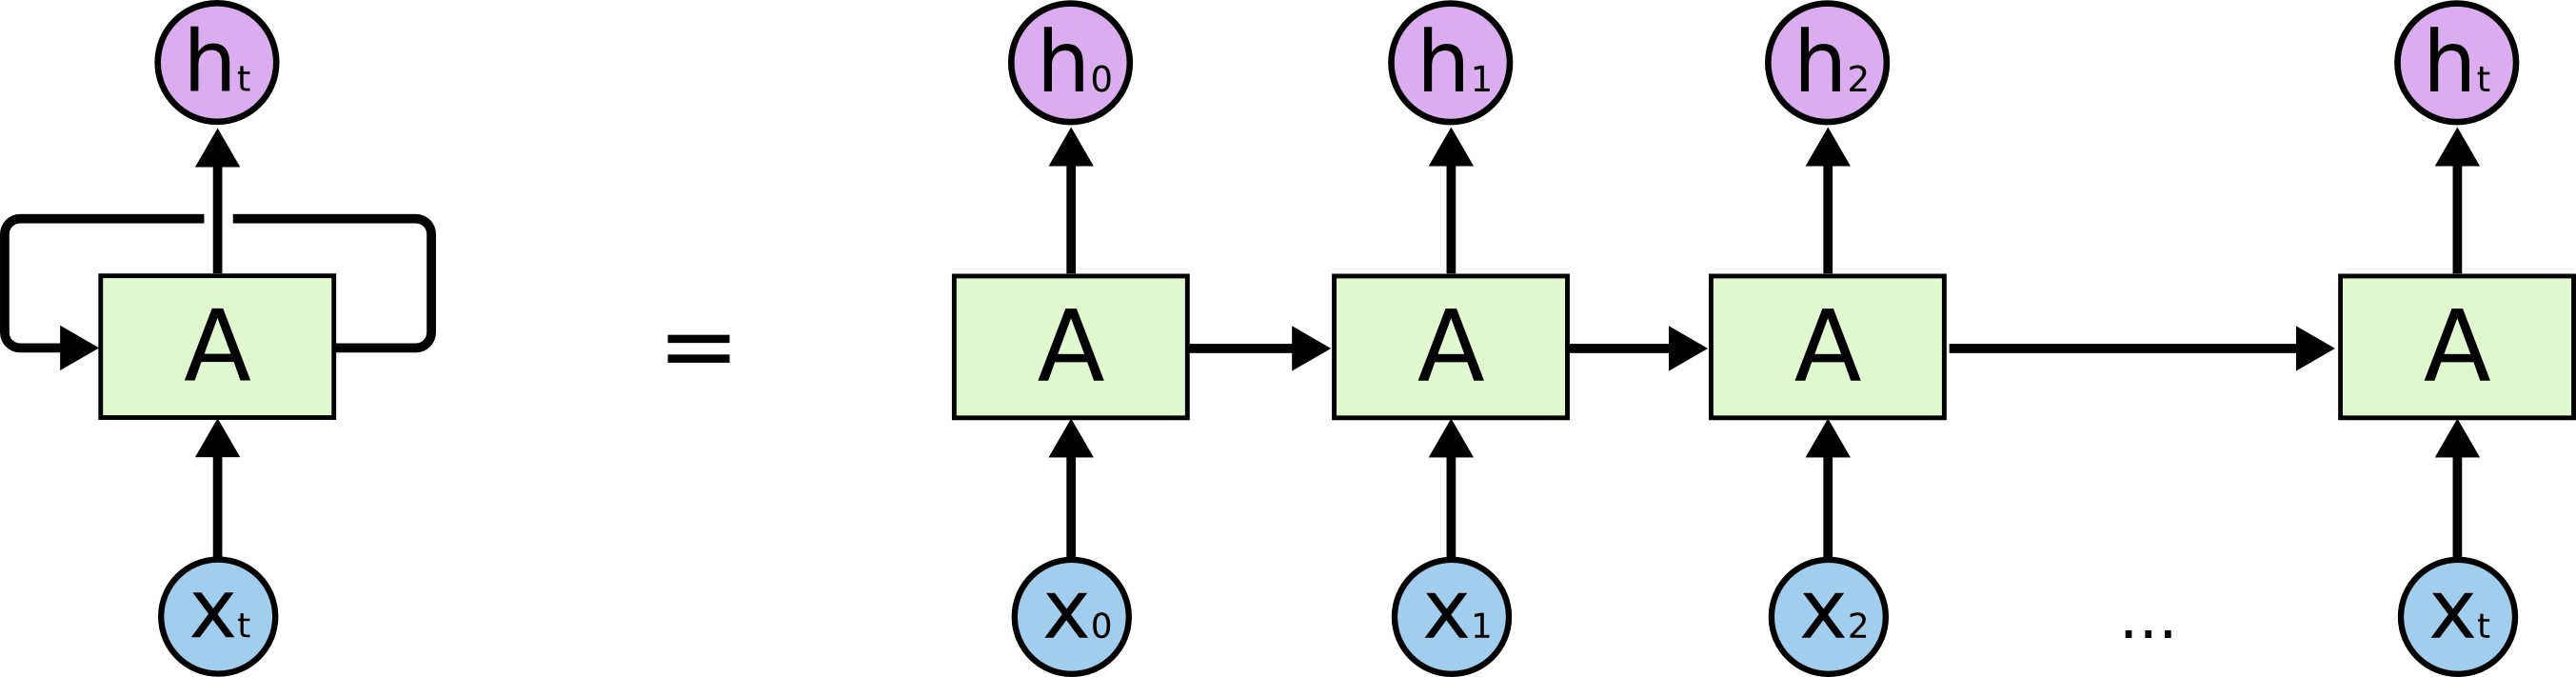
\includegraphics[width=\textwidth]{images/chapitre4/RNN-unrolled.png}
	\caption{Unrolled RNN (Understanding LSTM Networks, \url{https://colah.github.io/posts/2015-08-Understanding-LSTMs/)}}
	\label{fig:chap4:RNN_unroll}
\end{figure} 

\begin{align} \label{eq:LSTM}
	f_t &= \sigma_g(\mathbf{W}_f x_t + \mathbf{U}_fh_{t-1} + b_f)\\
	i_t &= \sigma_g(\mathbf{W}_i x_t + \mathbf{U}_ih_{t-1} + b_i)\\
	o_t &= \sigma_g(\mathbf{W}_o x_t + \mathbf{U}_oh_{t-1} + b_o)\\
	c_t &= f_t \circ c_{t-1} + i_t \circ \sigma_c(\mathbf{W}_cx_t + \mathbf{U}_c h_{t-1} + b_c)\\
	h_t &= o_t \circ \sigma_h (c_t)
\end{align}

\textbf{Figure \ref{fig:chap4:LSTM-gates}} shows how it works.

\begin{figure}
	\centering
	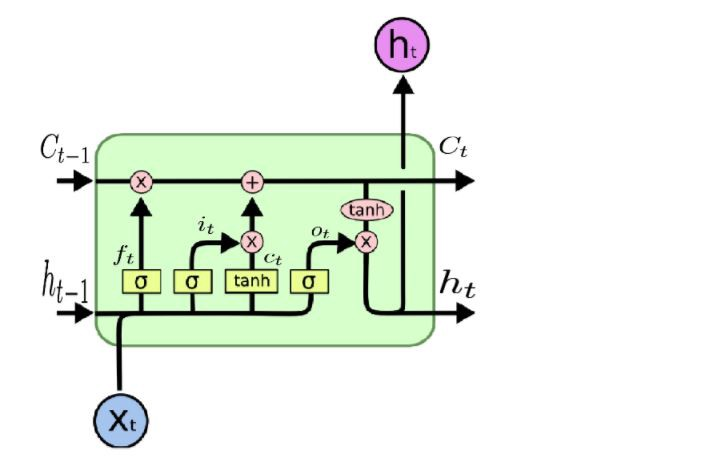
\includegraphics[width=0.6\textwidth]{images/chapitre4/LSTM1.jpeg}
	\caption{LSTM gates, \\ \url{https://hackernoon.com/understanding-architecture-of-lstm-cell-from-scratch-with-code-8da40f0b71f4)}}
	\label{fig:chap4:LSTM-gates}
\end{figure} 

A bidirectional LSTM works the same way, but the input is fed in the two direction, from the start to the end and from the end to the start.
\section{Attention Mechanism}
Attention mechanism\cite{zhou-etal-2016-attention,Vaswani2017AttentionIA} add an extra layer between LSTM outputs and the final output of the network. It merges word level features into sentence features using a weight vector. \\

\begin{figure}
	\centering
	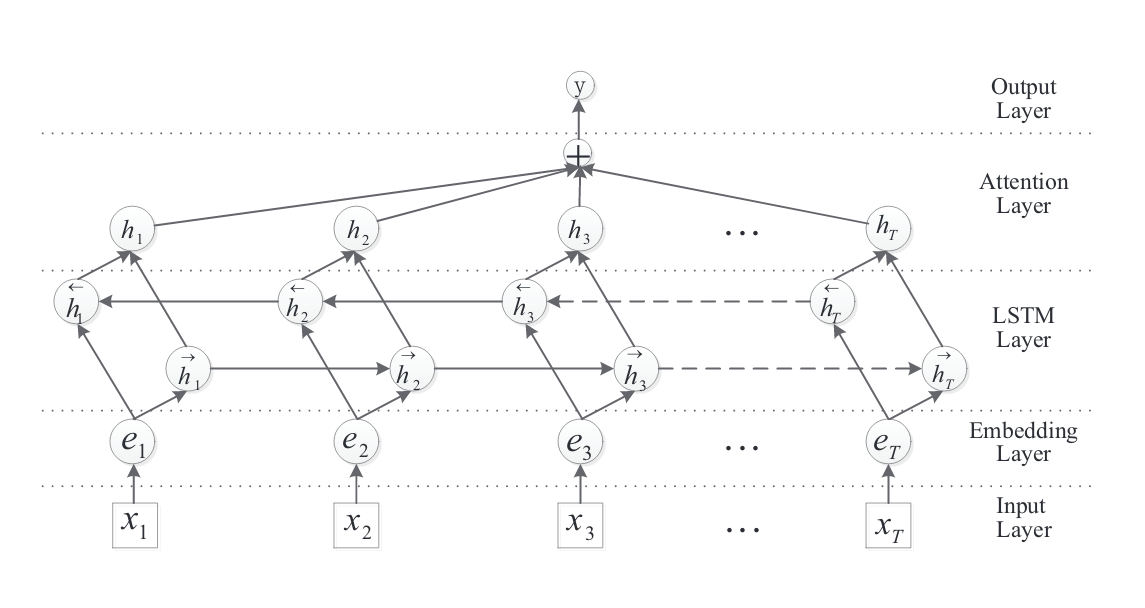
\includegraphics[width=\textwidth]{images/chapitre4/attention.png}
	\caption{Bidirectional LSTM model with Attention}
	\label{fig:chap4:attention}
\end{figure}

Outputs sequence of the LSTM are summed element-wise in order to merge them. We have that $h_i = [\overrightarrow{h_i} + \overleftarrow{h_i}]$, $\overrightarrow{h_i}$ and $\overleftarrow{h_i}$ begin the outputs i of sequence in each direction as show at \textbf{Figure \ref{fig:chap4:attention}}.\\

Let $H$ be a matrix of the concatenation of all the $h_i$, 
\begin{equation}
	H = [h_1,h_2,...,h_T]
\end{equation}
Where T is the sequence length. 

Then we define 
\begin{align}
	M &= \tanh(H)\\
	\alpha &= softmax(w^TM) \\
	r &= H \alpha^T 
\end{align}
Finaly, we compute $h^* = \tanh(r)$.

For the classification, it uses a softmax classifier as $\hat{p}(y|S) = softmax(W^Sh^* + b)$. Originaly the loss function is the negative log-likelihood, but as in this case it is a binary classification I used binary cross entropy. 
\section{Results}
\subsection{Methodology}
In order to train the models and perform hyper parameters optimization grid search have been used when it was possibile (on the liar-liar dataset) and knwoleadge aquiered there have been used in order to tune parameters for the networks on the \textbf{Fake News Corpus}. In addition, in order to find the bests parameters among all tested with gird search, for each metrics, the training epochs having the highest validation value for that metrics have been choosen. \\

As SMOTE cannot be used on the \textbf{Fake News Corpus} dues to the size of the corpus, in order to rebalance the dataset the minority class have been over sampled by feeding multiple times the same input by looping through them. 
\subsection{Liar-Liar dataset results}
As explained earlier, both models have been train using different embedding: the first one being pre-trained word2vec vectors of size 300 and the second one beging a tunable parameters with different embedding size.
\subsubsection{Using word2vec embedding}
